\documentclass[tikz, border=5mm]{standalone}
\usetikzlibrary{shapes.geometric, arrows.meta, positioning, calc, backgrounds, fit}

\begin{document}
	
	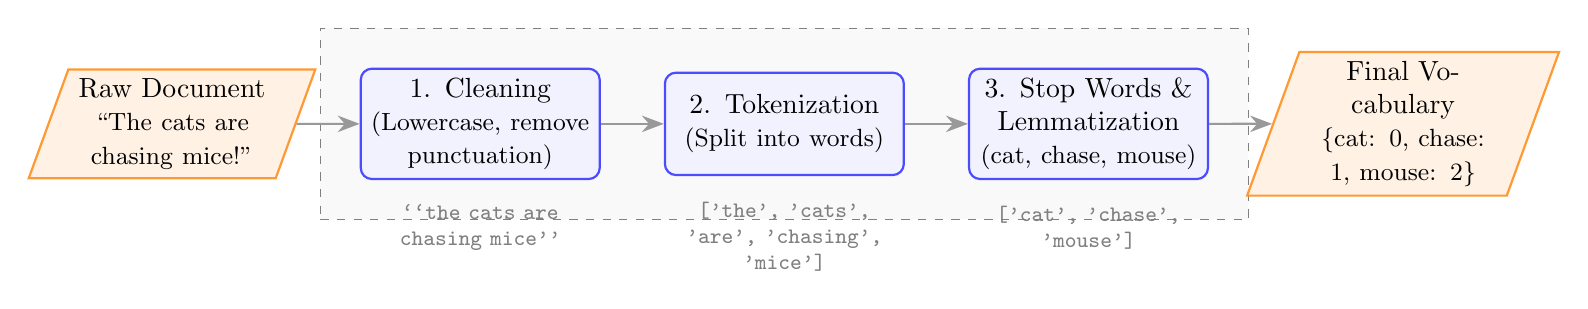
\begin{tikzpicture}[
		block/.style={
			rectangle, 
			draw=blue!70, 
			fill=blue!5, 
			thick, 
			text width=2.8cm, 
			align=center, 
			minimum height=1.3cm, 
			rounded corners
		},
		io/.style={
			trapezium, 
			trapezium left angle=70, 
			trapezium right angle=110, 
			draw=orange!80, 
			fill=orange!10, 
			thick, 
			text width=2.4cm, 
			align=center, 
			minimum height=1.3cm
		},
		arrow/.style={
			-{Stealth[scale=1.2]}, 
			thick, 
			draw=gray!80
		}
		]
		
		% Main nodes
		\node (doc) [io] {Raw Document\\ \small``The cats are chasing mice!''};
		\node (clean) [block, right=0.8cm of doc] {1. Cleaning\\ \small(Lowercase, remove punctuation)};
		\node (tokenize) [block, right=0.8cm of clean] {2. Tokenization\\ \small(Split into words)};
		\node (stop) [block, right=0.8cm of tokenize] {3. Stop Words \& Lemmatization\\ \small(cat, chase, mouse)};
		\node (vocab) [io, right=0.8cm of stop] {Final Vocabulary\\ \small\{cat: 0, chase: 1, mouse: 2\}};
		
		% Example labels below each step
		\node[below=0.2cm of clean, text width=2.8cm, align=center, font=\footnotesize\ttfamily\color{gray}] {``the cats are chasing mice''};
		\node[below=0.2cm of tokenize, text width=2.8cm, align=center, font=\footnotesize\ttfamily\color{gray}] {['the', 'cats', 'are', 'chasing', 'mice']};
		\node[below=0.2cm of stop, text width=2.8cm, align=center, font=\footnotesize\ttfamily\color{gray}] {['cat', 'chase', 'mouse']};
		
		% Connection arrows
		\draw [arrow] (doc) -- (clean);
		\draw [arrow] (clean) -- (tokenize);
		\draw [arrow] (tokenize) -- (stop);
		\draw [arrow] (stop) -- (vocab);
		
		% Background box for grouping the pipeline (Title removed)
		\begin{scope}[on background layer]
			\node[draw, dashed, color=gray, fill=gray!5, fit=(clean) (tokenize) (stop), inner sep=0.5cm] {};
		\end{scope}
		
	\end{tikzpicture}
	
\end{document}